\section{Training and Control}

\subsection{Early Stopping}

  Since neural networks are overparameterized, it makes sense that given enough training time, they will overfit to the training set. Therefore, you must stop training when the validation loss starts to decrease. This simple method is known as \textbf{early stopping}. 

\subsection{L1 and L2 Regularization}

  Another way to regularize is by simply adding in a L1 or L2 regularization term. 

  Sometimes, it may not always be the best idea to regularize a neural net equally through all weights. For example, weights which may be deeper down the forward pass may focus on more high level features and therefore should be regularized differently than those that are close to the input. Other types of regularization, such as Fiedler regularization \cite{tam2020fiedler} focuses on preserving the graph structure of the weights. 

\subsection{Dropout}

  Overfitting is always a problem. With unlimited computation, the best way to regularize a fixed-sized mdoel is to average the predictions of all possible settings of the parameters, weighting each setting by its posterior probability given the training the data. However, this is computationally expensive and cannot be done for moderately complex models. 

  The dropout method introduced by \cite{srivastava14a}, addresses this issue. We literally drop out some features (not the weights!) before feeding them to the next layer by setting some activation functions to $0$. Given a neural net of $N$ total nodes, we can think of the set of its $2^N$ thinned subnetworks. For each training minibatch, a new thinned network is sampled and trained. 

  At each layer, recall that forward prop is basically 
  \begin{align*}
      \mathbf{z}^{[l+1]} & = \mathbf{W}^{[l+1]} \mathbf{a}^{[l]} + \mathbf{b}^{[l+1]} \\
      \mathbf{a}^{[l+1]} & = \boldsymbol{\sigma} (\mathbf{z}^{[l+1]}) 
  \end{align*}
  Now what we do with dropout is 
  \begin{align*}
      r_j^{[l]} & \sim \mathrm{Bernoulli}(p) \\
      \Tilde{\mathbf{a}}^{[l]} & = \mathbf{r}^{[l]} \odot \mathbf{a}^{[l]} \\
      \mathbf{z}^{[l+1]} & = \mathbf{W}^{[l+1]} \Tilde{\mathbf{a}}^{[l]} + \mathbf{b}^{[l+1]} \\
      \mathbf{a}^{[l+1]} & = \boldsymbol{\sigma} (\mathbf{z}^{[l+1]}) 
  \end{align*}
  Basically we a sample a vector of $0$s and $1$s from a multivariate Bernoulli distribtion. We element-wise multiply it with $\mathbf{a}^{[l]}$ to create the thinned output $\Tilde{\mathbf{a}}^{[l]}$. In test time, we do not want the stochasticity of having to set some activation functions to $0$. That is, consider the neuron $\mathbf{a}^{[l]}$ and the random variable $\Tilde{\mathbf{a}}^{[l]}$. The expected value of $\mathbf{z}^{[l+1]}$ is 
  \[\mathbb{E}[\mathbf{z}^{[l+1]}] = \mathbb{E}[ \mathbf{W}^{[l+1]} \Tilde{\mathbf{a}}^{[l]} + \mathbf{b}^{[l+1]}] = \mathbb{E}[ \mathbf{W}^{[l+1]} \Tilde{\mathbf{a}}^{[l]}] = p \mathbb{E}[\mathbf{W}^{[l+1]} \mathbf{a}^{[l]}] \]
  and to make sure that the output at test time is the same as the expected output at training time, we want to multiply the weights by $p$: $W^{[l]}_{\text{test}} = p \, W^{[l]}_{\text{train}}$. Another way is to use \textbf{inverted dropout}, where we can divide by $p$ in the training stage and keep the testing method the same. 

  \begin{code} 
    The code \href{code/02_Training/dropout.ipynb}{here} shows how to implement dropout in PyTorch, which uses dropout layers. 
  \end{code}

\subsection{Data Augmentation}

  It is well known that having more training data helps with overfitting, and so we may be able to perform basic transformations to our current data to artificially generate more training data. For example, if we have images, then we can flip, crop, translate, rotate, stretch, shear, and lens-distort these images with the same label. 

\subsection{Normalization Layers} 

  Just like how we have to normalize our data before we input into a linear model, it may help to normalize the outputs of one layer of a neural net before we input it into the next layer. This is an engineer's method to help with the training process. There are two ways that we can generally normalize data. First is to normalize each sample, known as \textbf{layer normalization}, and the other way is to normalize the samples over the batch. 

  \begin{definition}[Layer Norm]
    Given some batched output data $X \in \mathbb{R}^{b \times \mathbf{d}}$, where $b$ represents the batch size and $\mathbf{d} = d_1 \times \ldots \times d_k$ the dimension of each sample, we can normalize each $x_i = X_{i, :}$ in the batch with \textbf{layer normalization} by 
    \begin{equation}
      x_i \mapsto \frac{x_i - \mathbb{E}[x_i]}{\sqrt{\Var[x_i] + \varepsilon}} \odot \gamma + \beta
    \end{equation}
    where $\gamma, \beta$ are learnable parameters that are the same shape as $x_i$. If $X$ is of dimension $b \times \mathbf{d}$, we must use \texttt{nn.LayerNorm(d)} since these are the sizes of the learnable parameters. 
  \end{definition}

  \begin{example}[Layer Norm]
    The following example shows that each row (sample in batch) is normalized independently from one another. 
    \begin{lstlisting}
      ln = nn.LayerNorm(5)
      x = torch.Tensor(range(10)).reshape(2, 5)
      print(x)
      tensor([[0., 1., 2., 3., 4.],
              [5., 6., 7., 8., 9.]])

      print(ln(x))
      tensor([[-1.4142, -0.7071,  0.0000,  0.7071,  1.4142],
              [-1.4142, -0.7071,  0.0000,  0.7071,  1.4142]],
             grad_fn=<NativeLayerNormBackward0>)
    \end{lstlisting}
    This also works for higher dimensions. 
    \begin{lstlisting}
      ln = nn.LayerNorm((5, 2))
      x = torch.Tensor(range(20)).reshape(2, 5, 2)
      print(x)
      tensor([[[ 0.,  1.],
               [ 2.,  3.],
               [ 4.,  5.],
               [ 6.,  7.],
               [ 8.,  9.]],

              [[10., 11.],
               [12., 13.],
               [14., 15.],
               [16., 17.],
               [18., 19.]]])
      print(ln(x))
      tensor([[[-1.5667, -1.2185],
               [-0.8704, -0.5222],
               [-0.1741,  0.1741],
               [ 0.5222,  0.8704],
               [ 1.2185,  1.5667]],

              [[-1.5667, -1.2185],
               [-0.8704, -0.5222],
               [-0.1741,  0.1741],
               [ 0.5222,  0.8704],
               [ 1.2185,  1.5667]]], grad_fn=<NativeLayerNormBackward0>)
    \end{lstlisting}
    The tunable parameters $\gamma, \beta$ are indeed the same size. They are initialized to $1$s and $0$s. 
      \begin{lstlisting}
      >>> for k, v in ln.state_dict().items(): 
      ...     print(k, v)
      ... 
      weight tensor([[1., 1.],
              [1., 1.],
              [1., 1.],
              [1., 1.],
              [1., 1.]])
      bias tensor([[0., 0.],
              [0., 0.],
              [0., 0.],
              [0., 0.],
              [0., 0.]])
    \end{lstlisting}
  \end{example}

  \begin{definition}[Batch Norm]
    \textbf{Batch normalization} targets each feature over all batches rather than each sample (like columns vs rows). Therefore, given some batched output data $X \in \mathbb{R}^{b \times \mathbf{d}}$, where $b$ represents the batch size and $\mathbf{d} = d_1 \times \ldots \times d_k$ the dimension of each output, we can normalize each feature $x_i = X_{:,i \in \mathbf{d}}$ by 
    \begin{equation}
      x_i \mapsto \frac{x_i - \mathbb{E}[x_i]}{\sqrt{\Var[x_i] + \varepsilon}} \odot \gamma + \beta
    \end{equation}
    where $\gamma, \beta \in \mathbb{R}^b$ are learnable parameters that are the same size as the batch. There are two types of batch norms implemented in pytorch. 
    \begin{enumerate}
      \item If $X$ has hyperdimension $2$ with $b \times d$, we use \texttt{BatchNorm1d(d)} since we are normalizing over the batch for each feature and we have $d$ features to normalize. 
      \item If $X$ has hyperdimension $3$ with $b \times d_1 \times d_2$, we use \texttt{BatchNorm1d(d\_1)}. 
      \item If $X$ has hyperdimension $4$ with $b \times d_1 \times d_2 \times d_3$, we use \texttt{BatchNorm2d(d\_1)}. 
    \end{enumerate}
  \end{definition}

  \begin{example}[Batch Norm 1D]
    We can see that each feature is normalized independently from one another. For 2D, 
    \begin{lstlisting}
      >>> bn = nn.BatchNorm1d(5)
      >>> x = torch.Tensor(range(10)).reshape(2, 5)
      >>> print(x) 
      tensor([[0., 1., 2., 3., 4.],
              [5., 6., 7., 8., 9.]])
      >>> print(bn(x))
      tensor([[-1.0000, -1.0000, -1.0000, -1.0000, -1.0000],
              [ 1.0000,  1.0000,  1.0000,  1.0000,  1.0000]],
             grad_fn=<NativeBatchNormBackward0>)
    \end{lstlisting}
    For 3D inputs, 
    \begin{lstlisting}
      >>> bn = nn.BatchNorm1d(5)
      >>> x = torch.Tensor(range(30)).reshape(2, 5, 3)
      >>> print(x) 
      tensor([[[ 0.,  1.,  2.],
               [ 3.,  4.,  5.],
               [ 6.,  7.,  8.],
               [ 9., 10., 11.],
               [12., 13., 14.]],

              [[15., 16., 17.],
               [18., 19., 20.],
               [21., 22., 23.],
               [24., 25., 26.],
               [27., 28., 29.]]])
      >>> print(bn(x))
      tensor([[[-1.1267, -0.9941, -0.8616],
               [-1.1267, -0.9941, -0.8616],
               [-1.1267, -0.9941, -0.8616],
               [-1.1267, -0.9941, -0.8616],
               [-1.1267, -0.9941, -0.8616]],

              [[ 0.8616,  0.9941,  1.1267],
               [ 0.8616,  0.9941,  1.1267],
               [ 0.8616,  0.9941,  1.1267],
               [ 0.8616,  0.9941,  1.1267],
               [ 0.8616,  0.9941,  1.1267]]], grad_fn=<NativeBatchNo
      rmBackward0>)
    \end{lstlisting}
  \end{example}

  \begin{example}[Batch Norm 2D]
    Here is an example of batch norm 2d. There really isn't a difference between these two methods except the dimension that they take in. That is all. 
    \begin{lstlisting}
      >>> bn = nn.BatchNorm2d(5)
      >>> x = torch.Tensor(range(60)).reshape(2, 5, 3, 2)
      >>> print(x) 
      tensor([[[[ 0.,  1.],
                [ 2.,  3.],
                [ 4.,  5.]],
                ...
                [58., 59.]]]])
      >>> print(bn(x))
      tensor([[[[-1.1592, -1.0929],
                [-1.0267, -0.9605],
                ...
                [ 1.0929,  1.1592]]]], grad_fn=<NativeBatchNormBack
      ward0>)
    \end{lstlisting}
  \end{example}

\subsection{Residual Connections} 

  \begin{figure}[H]
    \centering 
    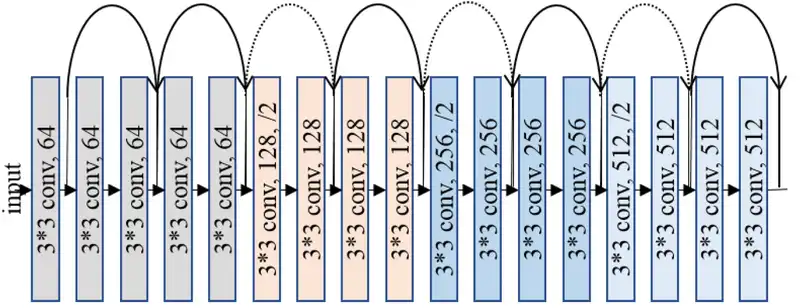
\includegraphics[scale=0.4]{img/02_Control/resnet_arch.png}
    \caption{Resnet architecture. } 
    \label{fig:resnet_arch}
  \end{figure}

  \begin{figure}[H]
    \centering 
    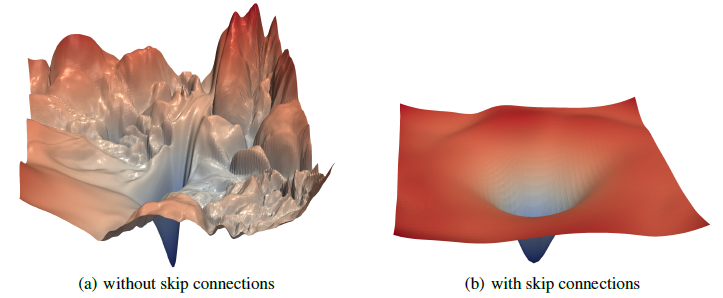
\includegraphics[scale=0.4]{img/02_Control/resnet_loss.png}
    \caption{Low-dimensional visual of loss with vs without residual connections. } 
    \label{fig:resnet_loss}
  \end{figure}

  \begin{figure}[H]
    \centering 
    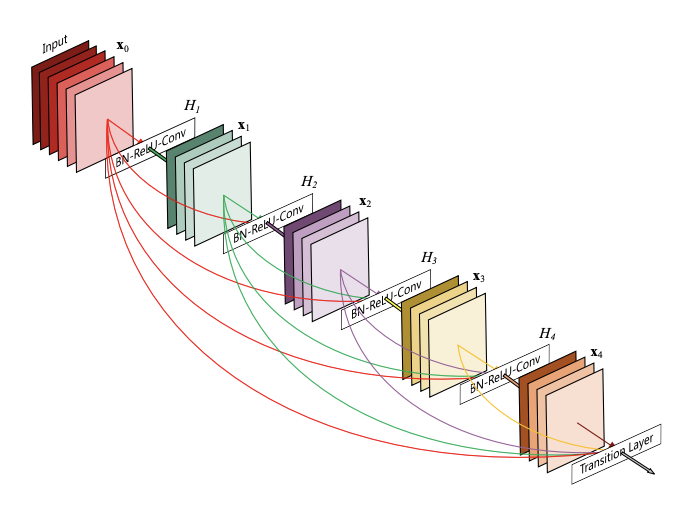
\includegraphics[scale=0.4]{img/02_Control/densenet.png}
    \caption{Densenet architecture. } 
    \label{fig:densenet_architecture}
  \end{figure}

\subsection{Network Pruning}

  It can be computationally and memory intensive to train and utilize neural networks. This is where network pruning comes in, which attempts to identify a subnetwork that performs as well as the original. Given a neural net $f(\mathbf{x}, \boldsymbol{\theta})$ where $\boldsymbol{\theta} \in \mathbb{R}^M$, a pruned neural network can be thought of as a subnetwork $f(\mathbf{x}, \mathbf{m} \odot \boldsymbol{\theta})$, where $\mathbf{m}$ is a \textbf{mask}, i.e. a vector in $\{0, 1\}^M$ that, when multiplied component-wise to $\boldsymbol{\theta}$, essentially ``deletes" a portion of the parameters. 
  \begin{center}
      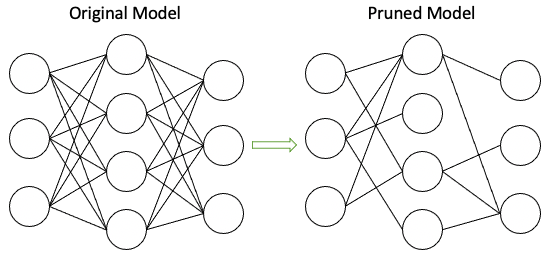
\includegraphics[scale=0.4]{img/02_Control/pruned_network.png}
  \end{center}
  This idea has been around for a long time, and the general method of pruning is as such: 
  \begin{enumerate}
      \item We initialize the neural network $f(\mathbf{x}, \boldsymbol{\theta}_0)$ and train it until we have $f(\mathbf{x}, \boldsymbol{\theta})$. 
      \item We now prune the network. The most basic pruning scheme is to keep the top $k\%$ largest weights, since smaller weights do not contribute much to the forward prop, and thus can be ignored. 
  \end{enumerate}
  These pruned networks have been shown to reach accuracies as high as the original network, with equal training progress. Now, if we were to take only this pruned network and train it from the beginning, it will perform as well as the original network, \textit{only under} the condition that we start from the same initialization $\mathbf{m} \odot \boldsymbol{\theta}$. If we take this subnetwork and initialize it differently at $\boldsymbol{\theta}_0^\prime$, then this subnetwork would not train well. Therefore, the performance of the pruned network is dependent on the initialization! 

  If we had initialized the full network differently, trained it, and then pruned again, we may have a different subnetwork that will only train well on its own given this new initialization. Therefore, a good initialization is extremely important for training subnetworks. This fact doesn't help much since we can't just take some arbitrary subnetwork and train it since we don't know the good initialization. We must always train the full network, then find the subnetwork, and then find its initialization. 

  This is essentially the \textbf{lottery ticket hypothesis} \cite{frankle2019lottery}, which states that a randomly-initialized, dense neural network contains a subnetwork that is initialized such that, when trained in isolation, it can match the test accuracy of the original network after training for at must the same number of iterations. 

  This paper hints at why neural networks work at all. It first states that only a very small subnetwork is responsible for the vast majority of its performance, but it must be initialized at the right position. But by overparameterizing these neural nets so much (by a certain margin), they have so many different combinations of subnetworks such that whatever initialization you throw at it, it is guaranteed that some subnetwork within it will train well with this initialization. This subnetwork is called the \textit{winning ticket}. 

\subsection{Curriculum Learning}

\subsection{Summary}

  Here is a few steps you can take as a guide to training a neural network. 
  \begin{enumerate}
    \item Preprocess the data. 
    \item Choose your neural net architecture (number of layers/neurons, etc.) 
    \item Do a forward pass with the initial parameters, which should be small, and check that the loss is reasonable (e.g. $\log(1/10) \approx 2.3$ for softmax classification of 10 classes). 
    \item Now crank up the regularization term, and your loss should have gone up. 
    \item Now try to train on only a very small portion of your data without regularization using SGD, which you should be able to overfit and get the accuracy to 100\%. 
    \item Now you can train your whole dataset. Start off with a small regularization (e.g. 1e-6) and find a learning rate that makes the loss go down. 
    \begin{enumerate}
        \item Run for a few epochs to see if the cost goes down too slowly (step size is too small) or the cost explodes (step size too big). A general tip is that if the cost is ever bigger than $3$ times the original cost, then this is an indication that the cost has exploded. 
        \item We can run a grid search (in log space) over the learning rate and the regularization hyperparameters over say 10 epochs each, and compare which one makes the most progress. 
    \end{enumerate}
    \item Monitor and visualize the loss curve. 
    \begin{center}
        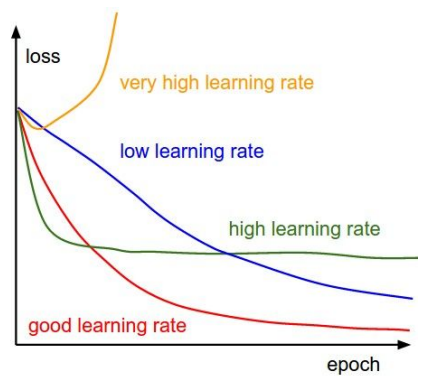
\includegraphics[scale=0.5]{img/02_Control/loss_curve_diagnostics.png}
    \end{center}
    If you see loss curves that are flat for a while and then start decreasing, then bad initialization is a prime suspect. 
    \item We also want to track the ratio of weight updates and weight magnitudes. That is, we can take the norm of the weights $\boldsymbol{\theta}$ and the gradient updates $\nabla \boldsymbol{\theta}$, and a rule of thumb is that the ratio should be about 
    \[\frac{||\nabla \boldsymbol{\theta}||}{||\boldsymbol{\theta}||} \approx 0.001 \text{ or } 0.01\]
  \end{enumerate}

